\chapter{Introduction}
\label{chapter:intro}
%The opening paragraph should motivate the central theme of the thesis. Exaplain what the core problem is, and why that's important. Bear in mind that this chapter is targeting a broard audience, so try to be as accessible as possible. 

Decision trees \cite{breiman2001random} and deep learning \cite{lecun2015deep} have become ubiquitous in the field of medical image processing. With the combination of the increasing volume of digitised imaging data and advances in both hardware and software,  these so-called ``black-box" machine learning (ML) algorithms have enabled a substantial leap in performace in a plethora of applications from image analysis to surgical assistance \cite{criminisi2013decision,litjens2017survey}. For certain well-defined tasks with access to homogeneous and carefully annotated data, such machine learning systems have begun to surpass the performance of clinical experts \cite{esteva2017dermatologist,gulshan2016development,rajpurkar2017chexnet,wu2019deep}. However, translation of these research innovations into clinical practice requires care. In medical imaging applications where the algorithm's outputs inform scientific conclusions in research, and diagnostic, prognostic or interventional decisions in clinics, we need principled protocols to ensure safety. 

In practice, ML systems often face situations where the correct decision or prediction is ambiguous. We therefore need a mechanism to quantify the confidence of the model output (e.g. error bounds) and act upon it to prevent catastrophic failures. We would also like to be able to reason about the sources of such uncertainty, and further improve the performance. Does the training data need to be more diverse? Were the images or the annotations too noisy? It might have been that the choice of the model was not adequate. Or perhaps we may have been just unlucky and the particular instance of failures is an inherently challenging case where the input image did not contain enough information. Implementing systematic approaches to answering these questions is important not only to improve the predictive performance, but also to build trust with the practioners. However, to date, the majority of deep learning and decision tree techniques used in the medical imaging context rely on deterministic methods, and lack a mechanism to communicate uncertainty, a key ingredient to address such problems. 

In contrast, \textit{probabilistic machine learning} provides a natural framework to quantify the degree of uncertainty over different variables of interest, be it the prediction, the model parameters and structures, or the underlying data (images and labels) \cite{ghahramani2015probabilistic}. Probability distributions are used to represent all the uncertain unobserved quantities in a model and how they relate to the data, and probability theory is used as a language to compute and manipulate these distributions. The main goal of this thesis is to develop a practical framework for medical imaging applications to model different types of uncertainty in neural networks and decision trees by translating ideas from the paradigm of probabilistic machine learning. In the process, several fundamental enhancements to current methods arise. 

\textcolor{red}{\textbf{Could include a couple of illustrative failure cases? } }



%The most widely used deep learning models have an important shortcoming: they lack an under- lying mechanism to provide uncertainty infor- mation about the predictions they make. Instead they often output point estimates between 0 and 1, which are often taken blindly as a measure of confidence. There have already been a few high profile cases where blindly trusting deci- sions made by deep learning algorithms has had disastrous consequences. For example in 2016, and then again in 2018, there were fatalities due to mistakes made by the perception system of autonomous vehicles. In health care a wrong decision can be a matter of life or death, and so being able to place trust in the decisions of deep learning models applied to such an industry is of critical importance.

% These questions are becoming more important to patient safety as many research groups and companies have deployed or are aiming to deploy ML technology in clinical practice.
%
%
% In practice, ML systems often face situations where the correct decision is ambiguous, and therefore principled mechanisms for quantifying uncertainty are required to envision potential practical deployment.

%
%
%
%\paragraph{Deep learning and decisions trees are ubiquitous in research:} 
%\begin{itemize}
%	\item Decision trees and deep learning have become ubiquitous in the field of medical image processing. The combination of the increasing volume of digitised imaging data and advances in both hardware and software enabled these high-performance machine learning models have lead to substantial progress in a wide range of applications ranging from image analysis to surgical assistance. 
%	\item Super-human performance for well-defined tasks when a large volume of clean data is available. 
%	\item Deployment in practice requires safety. Decting when the model fails. 
%\end{itemize}
%
%
%\paragraph{The importance of uncertainty quantification}
%\begin{itemize}
%	\item Many of the above problems are characterised by uncertainty. 
%	\item Probability theory provides a language for manipulating and representing these different types of uncertainty. 
%\end{itemize}
%
%\paragraph{Over-realiance on deterministic algorithms. }
%\begin{itemize}
%	\item To date, the current methods disproportionately focus on the performance and rely on deterministic algorithms. 
%	\item The central theme of the thesis to investigate ways to reason about different forms of uncertainty and assess the utility in different medical imaging applications.  
%\end{itemize}
%



%	\begin{enumerate}
%		\item The omission of clinical-practice guidelines produced a machine learning algorithm suggesting that respiratory infections are a leading cause of chest pain, completely omitting cardiac causes
%		\item An algorithm developed to help detect melanoma, for instance, should be derived from a sufficiently diverse sample; when these data aren’t used or aren’t available, algorithms run the risk of overlooking disease in underrepresented patient populations. 
%		\item Clinically important variables and endpoints should be present and robust, but this remains a challenge in many data resources. 
%\end{enumerate} }
%\textcolor{red}{\textbf{Explain through an example to illustrate the importance of uncertainty modelling?
%Quantifying risks, understand the sources of uncertainty and point to solutions. Pneumonia risk prediction? }}


%Deep learning and decisions trees are now ubiquitous in the field of medical image processing. However, the current methods disproportionately rely on deterministic algorithms, which lack a mechanism to represent and manipulate uncertainty about models and predictions. In safety-critical applications such as medical imaging, quantifying what the model does not know is important for constructing a reliable decision making system. The aim of this thesis is to explore probabilitic modelling as a framework to integrate uncertainty information in deep learning and decision tree models, and demonstrate utility in various medical image processing applications. 
%
%\textcolor{red}{
%	I should end with a clear goal statement. Examples from two notable theses are below:
%	\begin{itemize}
%		\item (David Mackay): ``The main goal of this thesis is to provide an objective and practical framework for the use of neural network techniques by applying the methods of Bayesian model comparison. In the process several enhancements to current neural network methods arise.''
%		\item (Yarin Gal): ``The main goal of this thesis is to develop such practical tools to reason about uncertainty in deep learning.''
%\end{itemize}}

 \section{Taxonomy of uncertainty}
There are many different types of uncertainty that are of practical importance. Here we provide a taxonomy of such uncertainty ``species'' and explain their relations and differences. 

Imagine you have a machine learning model, $F$, which takes some input $\mathbf{x}$  (e.g. a MR image) and makes a prediction or decision about the quantity of interest, $\mathbf{y}=F(\mathbf{x})$ (e.g. presence of pathology). %Here $\theta$ denotes the set of parameters of the model, and has been optimised based on training data, consisting of $N$ pairs of inputs and labels of interest $\mathcal{D} = \{\mathbf{x}_{i}, \mathbf{y}_i\}_{i=1}^N $.
You now have thoroughly evaluated the performance of the model on a held-out test dataset (e.g. a large public imaging dataset), and are about to deploy it in the wild (e.g. your local hospital). 

\textit{Predictive uncertainty} describes the degree of ambiguity (or confidence) in the model's prediction on an given input. For example, error bounds are a common measure of predictive uncertainty, and can be used to assess the reliability of prediction for the particular data instance at hands. You might be interested in knowing how well your model performs in a new environment, but you may not have access to a sufficient volume of ground-truth labels for validation. However, quantification of predictive uncertainty provides a proxy measure of performance on each data point, which can be used to manage failure risks in a principled way---if the model encouters input examples with overly high predictive uncertainty, then we should not trust the system. 

One is often interested not only in quantifying the predictive uncertainty, but also understanding its \textit{sources}. Having quantitative answers to questions such as ``is the model uncertain on this particular image because the observed feature is not represented in the training data or the image quality is too low to make conclusive decisions? Perhaps the current model does not best explain the data and we should use a different one?'' has clear benefits for building a more realiable system. Commonly, such \textit{source} uncertainty is divided into two types,\textit{aleatoric} and \textit{epistemic} uncertainty \cite{hora1996aleatory}. Aleatoric uncertainty --- from the Latin word, \textit{alea}, meaning a ``die'' --- refers to uncertainty about inherently stochastic phenomenon, . Epistemic uncertainty — from the Greek word \textit{episteme}, meaning “knowledge” — refers to uncertainty arising from lack of knowledge. \textcolor{red}{Elaborate on both with examples! Also, end }

\begin{figure}[bt]
	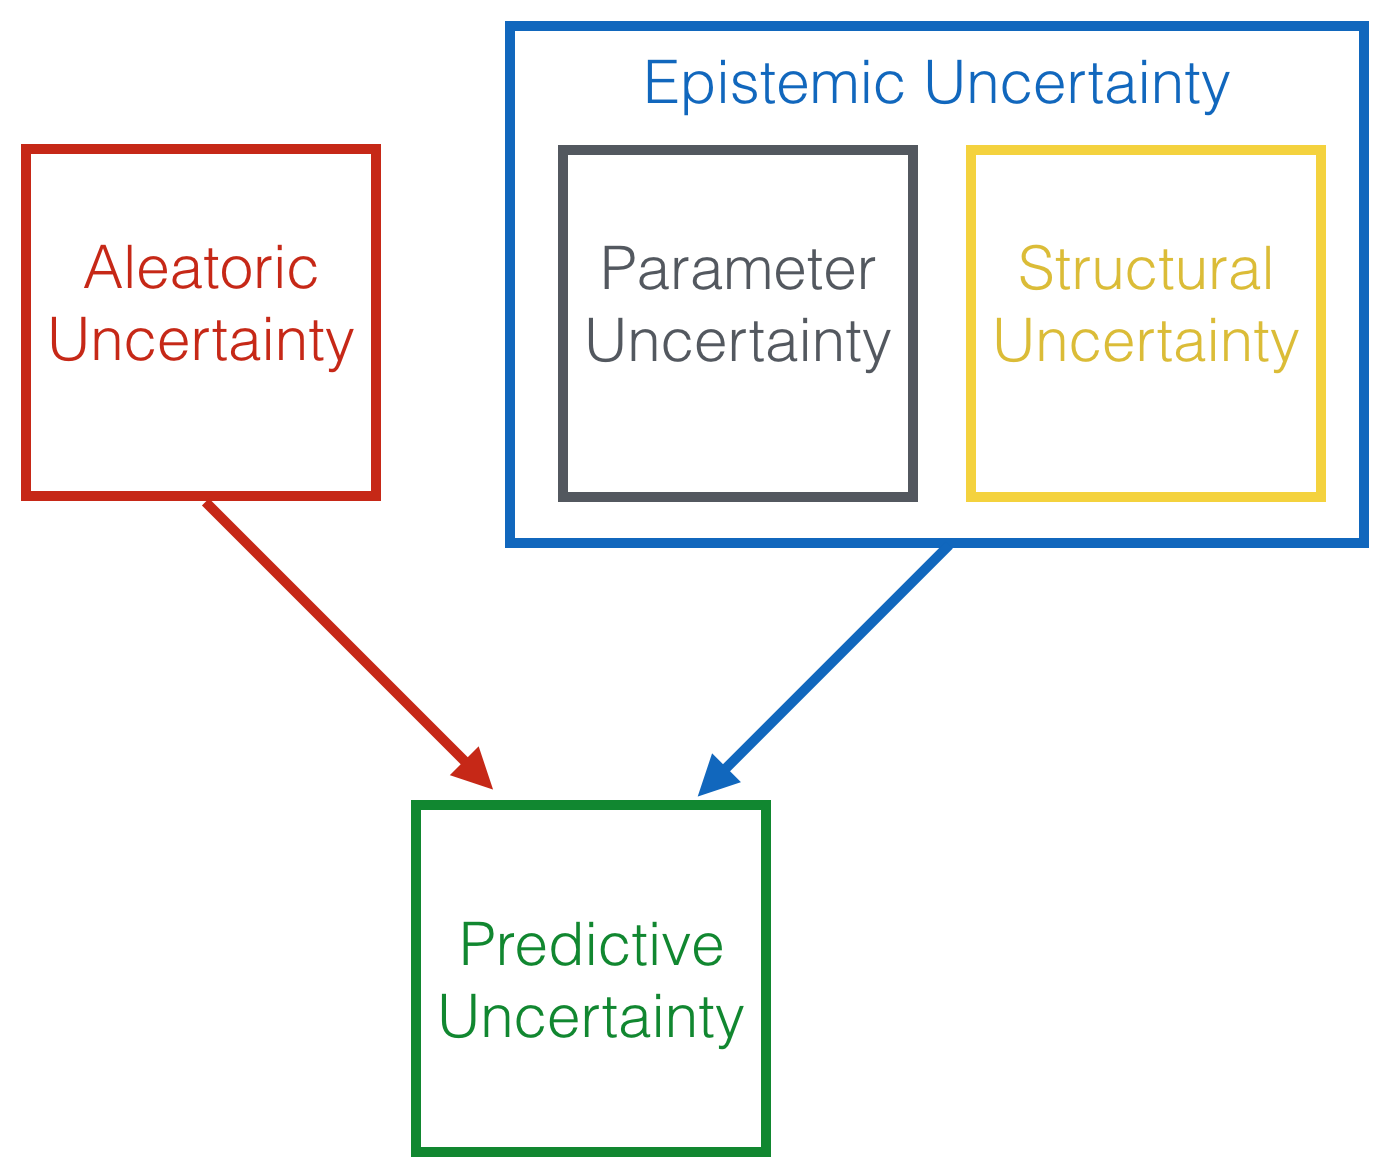
\includegraphics[width=0.5\linewidth]{chapter_1/uncertainty_taxonomy.png}
	\centering	
	%	\vspace{-2mm}
	\caption{Illustration of different types of uncertainty. The combined effects of both aleatoric and epistemic uncertainties induce \textit{predictive uncertainty}, the degree of confidence in a prediction of the model.  } 
	\label{fig:uncertainty_taxonomy}
	%\vspace{-10pt}
\end{figure}
 
%The model may encouter some unfamiliar inputs, which are not observed in the training data (e.g. a rare pathology).
% 

 
%More abstractly, the below are the types of uncertainty that the prior methods have tried to account for: 
%\begin{itemize}
%	\item Aleatory (intrinsic) uncertainty
%	\item Parameter uncertainty. 
%	\item Structural uncertainty. 
%\end{itemize}



% (From Sullivan 2015): It is common to divide uncer- tainty into two types, aleatoric and epistemic uncertainty. Aleatoric uncer- tainty — from the Latin alea, meaning a die — refers to uncertainty about an inherently variable phenomenon. Epistemic uncertainty — from the Greek ε`πιστη ́μη, meaning knowledge — refers to uncertainty arising from lack of knowledge. If one has at hand a model for some system of interest, then epis- temic uncertainty is often further subdivided into model form uncertainty, in which one has significant doubts that the model is even ‘structurally correct’, and parametric uncertainty, in which one believes that the form of the model reflects reality well, but one is uncertain about the correct values to use for particular parameters in the model

%Different areas of applications in medical imaging have studied to varying degrees ways to represent these types of uncertainty, which I elaborate in the remaining part of this section. 
%
%\textcolor{red}{Explain more fundamentally how probabilistic modelling provides a language to manipulate uncertainty about models and predictions. Read Zoubin's paper? This would be more of a background materials though. I guess we could come up with a very simple example to illustrate all these aspects? Perhaps augment Zoubin's example?}




\section{Uncertainty Modelling in Medical Imaging}
% I would like to use this section to motivate the importance of uncertainty quantification in medical imaging applications. 
The importance of representing uncertainty information has long been recognised in the medical imaging community. There is a large body of prior research on uncertainty quantification based on traditional probabilistic modelling techniques (e.g. graphical models and fuzzy logic) in a variety of medical image analysis applications such as registration, classification, segmentation and image synthesis. To the best of my knowledge, research addressing this issues goes back to the early 1970s. Here I provide a brief survey of such prior works.
 
 % (Yingzhen says):
 
 % (Ghahramani says):
 
 % (Yarin says): This probabilistic view of machine learning offers confidence bounds for data analysis and decision making, information that a biologist for example would rely on to analyse her data, or an autonomous car would use to decide whether to brake or not. In analysing data or making decisions, it is required to be able to tell whether a model is certain about its output, being able to ask “maybe I need to use more diverse data? or change the model? or perhaps be careful when making a decision?”. Such questions are of fundamental concern in Bayesian machine learning, and have been studied extensively in the field [Ghahramani, 2015]. 
 
% (Mackay says:) Bayesian probability theory provides a framework for inductive inference which has been called ‘common sense reduced to calculation’; it is a poorly known fact that Bayesian methods actually embody Occam’s razor automatically and quantitatively [26, 38].

\subsection{Computer-aided diagnosis}


\subsection{Synethesis}


\subsection{Registration}
\textbf{(Wells 2018 MICCAI)}: ``Probabilisitc image registration (PIR) literature conventionally quantifies the registration un- certainty by summary statistics of the transformation distribution. Previous researchers have found applications of various summary statistics: the Shannon entropy and its variants of the categorical transformation distribution were used to measure the registration uncertainty of DPR [6]; the variance [4,11,13], stan- dard deviation [10], inter-quartile range [5,15] and the covariance Frobenius norm [9] of the transformation distribution were used to quantify the registration un	certainty of CPR.''

\textbf{(Chapter 6 in Ivor Simpson's thesis):} "Registration Derived Uncertainty" describes how the uncertainty could be used in the downstream tasks. 

\subsection{Segmentation}
Eugnio mentioned in his paper 2013 \cite{iglesias2011combining} that "most approaches to joint segmentation of multiple structures rely on registration (i.e. by deforming an atlas (or a set thereof) to the target scan)". A very different approach from the mindless end-to-end learning that's so prevalent nowadays!  

(\textbf{Need to read}): Karl Friston's unified segmentation paper, Eugenio's MCMC based segmentation paper, and 

\textbf{(Claudia Blaiotta): } "One of the most significant advantages of variational inference over maximum likelihood estimation is its intrinsic capability of containing the effects of overfitting (Attias, 1999; Bishop, 2006). In the case of mixture models this allows, for instance, determining the optimal number of components (K) without performing cross-validation, which is usually rather demanding for the amount of computation, as well as for the amount of data, that it requires (Bishop, 2006)."

See Sec 5.2. (Page 106) "Advantages and challenges of Bayesian inference” where she comments that 
"In practice, this also means that explicit confidence measures cannot be directly obtained for the estimated parameters, which is a significant drawback for potential clinical applications, where the risk of error or failure needs to be accurately assessed and quantified.” 

Read "Juan Eugenio Iglesias, Mert Rory Sabuncu, and Koen Van Leemput. Incorporating parameter uncertainty in Bayesian segmentation models: Application to hippocampal subfield volumetry. In Proc. International Conference on Medical Image Computing and Computer Assisted Intervention, MICCAI 2012, pages 50–57. Springer, 2012b. "

\subsection{Inverse Problems}

\section{What is currently lacking?}
\textbf{We need to highlight that given a large quantity of clean training data, deep learning is capable of attaining extremely good performance. } In the last few years, deep learning techniques have permeated the field of medical image processing \cite{shen2017deep,litjens2017survey}. Beyond the automation of existing radiological tasks--- e.g. segmentation \cite{kamnitsas2017efficient}, detection \cite{roth2014new}, disease grading and classification \cite{araujo2017classification}---deep learning has been applied to a diverse set of ``data enhancement'' problems. Data enhancement aims to improve the quality, the information content, or the quantity of medical images available for research and clinics by transforming images from one domain to another \cite{isola2017image}. Previous research has shown the efficacy of data enhancement in different forms such as super-resolution \cite{oktay2016multi,chen2018efficient,ravi2019adversarial}, image synthesis \cite{nie2016estimating,kang2017deep}, denoising \cite{benou2017ensemble,chen2017low}, data harmonisation \cite{karayumak2018harmonizing,tax2019cross} across scanners and protocols, reconstruction \cite{sun2016deep,jin2017deep,hammernik2018learning,schlemper2018deep,zhu2018image,yang2018dagan,yoon2019efficient}, registration \cite{sokooti2017nonrigid,balakrishnan2018unsupervised} and quality control \cite{wu2017fuiqa,esses2018automated}.  These advances have the potential not only to enhance the quality and efficiency of radiological care, but also facilitate scientific discoveries in medical research through increased volume and content of usable data. 

\textbf{Surge of black-box models in medical imaging}: In the last few years, with increasing availability of labelled data, hardware and user-friendly software, black-box models such as deep learning and decision trees have permeated every corner of medical image processing research, often surpassing the performance of more traditional probabilistic techniques. 

However, the disproportionate majority of approaches rely on deterministic methods, which lack a mechanism to represent and manipulate uncertainty about models and predictions. In safety-critical applications such as medical imaging, quantifying what the model does not know is important for constructing a reliable decision making system. The aim of this thesis is to explore probabilitic modelling as a framework to integrate uncertainty information in deep learning and decision tree models, and demonstrate utility in various medical image processing applications. 
 
\textcolor{red}{The aim of the thesis is to investigate ways to } 

 
\section{Gap between the modern ML and medical imaging}
\textbf{Uncertainty in black-box models}: This section will review both theoretical and application-driven previous research on uncertainty modelling in deep learning and decision trees. We will discuss why such research is important for designing safe and interpretable systems for medical applications. 

\textcolor{red}{\textbf{Technical scope:} Here I should try and limit the scope by clearly explaining that the thesis focuses on simple supervised discriminative models, while touching upon other important avenues of research i.e.  generative, marriage between discriminative and generative, reinforcement learning (?), etc. We could use Eugenio's this year's MICCAI paper as a good example of hybrid models. }

\textcolor{red}{\textbf{Application scope:}  should also mention that the thesis focuses on tasks of processing high-dimensional image data that arise in medical settings. However, in fact, healthcare domain offers much richer array of data such as sensors, genomics, EHRs, and etc \cite{esteva2019guide}, which are outside the scope of the thesis. This link also has a few relevant references \href{https://www.mckinsey.com/industries/pharmaceuticals-and-medical-products/our-insights/machine-learning-and-therapeutics-2-0-avoiding-hype-realizing-potential}{link}.}




\section{Summary of the contributions} 
Here may be I should try and limite the scope of the thesis (perhaps earlier on? not sure)

To summarise, the contributions of this thesis are as follows:

\begin{enumerate}
	\item \textbf{Modelling predictive uncertainty}:  We introduce methods to quantify uncertainty over the output of deep learning and decision tree models. We demonstrate how such uncertainty measure can be used to quantify the quality of output and develop a more risk-averse image enhancement system for diffusion MRI \cite{tanno2016bayesian,tanno2017bayesian,tannonimg2019}.  We further show that the same concept could be naturally extended to the multi-task learning paradigm, and test the benefits in the context of MR-only radiotherapy planning application \cite{bragman2018multi}. 
	
	\item \textbf{Modelling human uncertainty}: We propose a method to model the biases and skill levels of human annotators, and integrate this information into the learning process of the neural network classifier \cite{tanno2019learning}. We demonstrate in classification of ultrasound cardiac images that the method not only improves the robustness of the model to label noise, but also yields insights into the performance of different human annotators. \textcolor{red}{Here we couls also mention briefly the ideal observer performance as a historical attempt to quantify the maximum possible accuracy.}
	
	\item \textbf{Modelling structural uncertainty}: We propose methods to learn model structures of a deep neural network. In the context of multi-task learning, we introduce the concept of \emph{stochastic filter  groups} (SFGs) \cite{sfg2019} to estimate the posterior distribution over the possible connectivity structures in a convolutional neural network in order to disentangle task-specific and shared features across different tasks. We demonstrate in the MR-only radiotherapy planning application that SFGs are capable of learning meaningful separations of representations, and consequently improve the performance. Lastly, we explore how the training algorithm of decision trees could be extended to adapt the architecture of a neural network to the given availability of training data and the complexity of the task \cite{AdaptiveNeuralTrees19}. 
	
\end{enumerate}

\section{Thesis Structure}